\documentclass[12pt,letterpaper,titlepage]{report}
\usepackage{algorithm2e}
\usepackage{listings}
\usepackage{geometry}
\usepackage{graphicx}
\usepackage[hypertexnames=false, pdftex]{hyperref}
%%%%%%%%%%%%%%%%%%%%%%%%%%%%%%%%%%%%%%%%%%%%%%%%%%%%%%%%%%%%%%%%%%%%
% use:$ pdflatex ScalFmmStarpu.tex
%%%%%%%%%%%%%%%%%%%%%%%%%%%%%%%%%%%%%%%%%%%%%%%%%%%%%%%%%%%%%%%%%%%%
\author{Berenger Bramas}
\title{A parallel FMM implementation using Starpu runtime (Draft)}
\date{November 17, 2011}
%% Package config
\lstset{language=c++, frame=lines}
\restylealgo{boxed}
\geometry{scale=0.8, nohead}
\hypersetup{ colorlinks = true, linkcolor = black, urlcolor = blue, citecolor = blue }
%% Remove introduction numbering
\setcounter{secnumdepth}{-1}
%%%%%%%%%%%%%%%%%%%%%%%%%%%%%%%%%%%%%%%%%%%%%%%%%%%%%%%%%%%%%%%%%%%%
%%%%%%%%%%%%%%%%%%%%%%%%%%%%%%%%%%%%%%%%%%%%%%%%%%%%%%%%%%%%%%%%%%%%
\begin{document}
\maketitle{}
\newpage
\tableofcontents
\newpage
%%%%%%%%%%%%%%%%%%%%%%%%%%%%%%%%%%%%%%%%%%%%%%%%%%%%%%%%%%%%%%%%%%%%
%%%%%%%%%%%%%%%%%%%%%%%%%%%%%%%%%%%%%%%%%%%%%%%%%%%%%%%%%%%%%%%%%%%%
\section{Abstract}
We introduce a novel approach of the Fast Multipole Method to be executed on heterogeneous platform.
Our implementation is supported by a runtime called Starpu[].
The current application can run on both shared and distributed memory model and makes Starpu responsible of the tasks management and scheduling.
We achieve good performances even if our tasks have an extremely small granularity.
%%%%%%%%%%%%%%%%%%%%%%%%%%%%%%%%%%%%%%%%%%%%%%%%%%%%%%%%%%%%%%%%%%%%
%%%%%%%%%%%%%%%%%%%%%%%%%%%%%%%%%%%%%%%%%%%%%%%%%%%%%%%%%%%%%%%%%%%%
\section{Introduction}
Super computers are mostly different from each other.
Looking at the top500 shows that some computers use GPUs some others do not, some are using quad-core and some others octa-core.
Several researches are done to propose to the programmer tools with the objective to bypass the architecture model when he creates an application.
One of the solutions is to use a runtime and letting this system scheduling the work depending on the architecture specificity.
Using such model require to rearrange the problem and express it differently.
Even if there are similarities between parallel/distributed and runtime programming approach, going from one to the other requires work especially if we want to achieve good performances.
In the other hand, using a runtime lets us focusing on the algorithm and delegates tasks organization.
%%%%%%%%%%%%%%%%%%%%%%%%%%%%%%%%%%%%%%%%%%%%%%%%%%%%%%%%%%%%%%%%%%%%
%%%%%%%%%%%%%%%%%%%%%%%%%%%%%%%%%%%%%%%%%%%%%%%%%%%%%%%%%%%%%%%%%%%%
\chapter{Introducing the FMM Algorithm}
\section{The FMM steps}
We are not going to describe the entire FMM, there are good papers that detail this subject since twenty years. Here, we give a quick overview of the FMM algorithm.
We can decompose the FMM in several distinct steps and mark a difference between cells and particles.
The Particles.
A particle has to be used for three steps:
Data from the source particles has to be transferred to its parent cell (P2M), and later this cell has to transfer back data to particles (L2P).
Also, each particle has to compute the direct interaction with its very close neighbors (P2P).
These two steps can be performed in parallel but the L2P and the P2P write to same memory part.
A leaf is composed by a cell and a group of particles.
\begin{figure}[h!]
\begin{center}
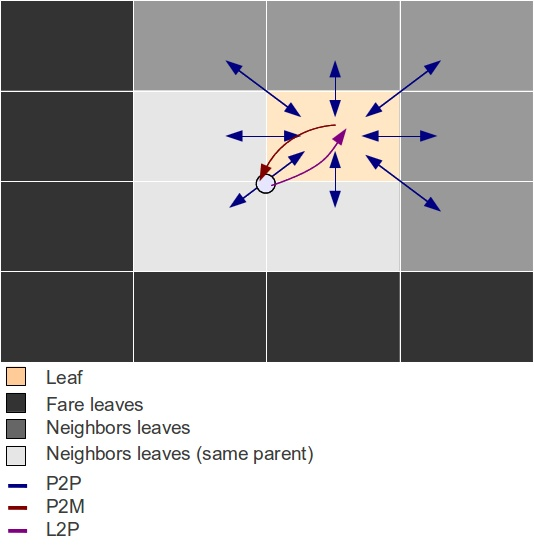
\includegraphics[width=12cm, height=12cm, keepaspectratio=true]{particles.jpg}
\caption{Particles operations}
\end{center}
\end{figure}
The Cells.
Each cell has to wait data from its child (M2M) to be able to transfer this data to its parent (M2M) and to use this same data for a computation with its interaction neighbors (M2L).
This same computation is also made in reverse from its interaction neighbors to this cell (M2L).
Finally it has to transfer data from its parents (L2L) and to transfer data to its child (L2L).
\begin{figure}[h!]
\begin{center}
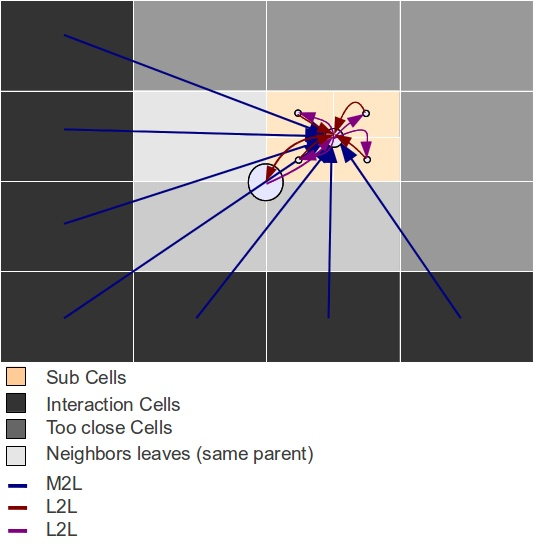
\includegraphics[width=12cm, height=12cm, keepaspectratio=true]{cells.jpg}
\caption{Cells operations}
\end{center}
\end{figure}
%%%%%%%%%%%%%%%%%%%%%%%%%%%%%%%%%%%%%%%%%%%%%%%%%%%%%%%%%%%%%%%%%%%%
%%%%%%%%%%%%%%%%%%%%%%%%%%%%%%%%%%%%%%%%%%%%%%%%%%%%%%%%%%%%%%%%%%%%
\chapter{Simple FMM implementation}
\section{Sequential}
The more basic approach to perform the steps of the FMM is to compute all operators one after the others.
Each operator required a loop over the cells at one or every levels of the tree.
Then, we only need to be careful about operators order in a general view.
For example, we can perform an upward pass (P2M, M2M), the M2L, the downward pass (L2L, L2P) and then the direct pass (P2P) even if the direct interactions can be computed at any time.
\BlankLine
\begin{algorithm}[H]
\restylealgo{boxed}
\linesnumbered
\SetLine
\BlankLine
\ForAll{Leaf lf in tree}{
        P2M( lf.cell , lf.particles )\;
}
\BlankLine
\caption{P2M}
\end{algorithm}
\BlankLine
\begin{algorithm}[H]
\restylealgo{boxed}
\linesnumbered
\SetLine
\BlankLine
\For{idxLevel $\leftarrow$ $Height - 2$ \KwTo 1}{
        \ForAll{Cell cl at level idxLevel}{
                M2M(cl, cl.child)\;
        }
}
\BlankLine
\caption{M2M}
\end{algorithm}
\BlankLine
\begin{algorithm}[H]
\restylealgo{boxed}
\linesnumbered
\SetLine
\BlankLine
\For{idxLevel $\leftarrow$ $Height - 1$ \KwTo 1}{
        \ForAll{Cell cl at level idxLevel}{
                neighbors $\leftarrow$ tree.getBoxInteractions( cl , idxLevel)\;
                M2L( cl, neighbors)\;
        }
}
\BlankLine
\caption{M2L}
\end{algorithm}
\BlankLine
\begin{algorithm}[H]
\restylealgo{boxed}
\linesnumbered
\SetLine
\BlankLine
\For{idxLevel $\leftarrow$ 1 \KwTo $Height - 2$}{
        \ForAll{Cell cl at level idxLevel}{
                L2L(cl, cl.child)\;
        }
}
\BlankLine
\caption{L2L}
\end{algorithm}
\BlankLine
\begin{algorithm}[H]
\restylealgo{boxed}
\linesnumbered
\SetLine
\BlankLine
\ForAll{Leaf lf in tree}{
        L2P( lf.cell , lf.particles )\;
}
\BlankLine
\caption{L2P}
\end{algorithm}
\BlankLine
\begin{algorithm}[H]
\restylealgo{boxed}
\linesnumbered
\SetLine
\BlankLine
\ForAll{Leaf lf in tree}{
        neighbors $\leftarrow$ tree.getLeavesInteractions( lf )\;
        P2P( lf, neighbors)\;
}
\BlankLine
\caption{P2P}
\end{algorithm}
\BlankLine
Also, it is possible to perform things a little differently by computing the M2L at each level just before the L2L.
\BlankLine
\begin{algorithm}[H]
\restylealgo{boxed}
\linesnumbered
\SetLine
\BlankLine
\For{idxLevel $\leftarrow$ 1 \KwTo $Height - 2$}{
        \ForAll{Cell cl at level idxLevel}{
                neighbors $\leftarrow$ tree.getBoxInteractions( cl , idxLevel)\;
                M2L( cl, neighbors)\;
                L2L( cl, cl.child )\;
        }
}
\ForAll{Cell cl at level $Height - 1$}{
        neighbors $\leftarrow$ tree.getBoxInteractions( cl , $Height - 1$)\;
        M2L( cl, neighbors)\;
	Leaf lf as cl\;
	L2P( cl , lf.particles )\;
}
\BlankLine
\caption{M2M \& M2L}
\end{algorithm}
\BlankLine
From this first serial approach we can imagine a straightforward task-based implementation.

Remark: we do not detail how the P2P can be computed in parallel in this document.

%%%%%%%%%%%%%%%%%%%%%%%%%%%%%%%%%%%%%%%%%%%%%%%%%%%%%%%%%%%%%%%%%%%%
%%%%%%%%%%%%%%%%%%%%%%%%%%%%%%%%%%%%%%%%%%%%%%%%%%%%%%%%%%%%%%%%%%%%
\section{A task oriented implementation}
We use OpenMP in our example.
The key idea is to understand that for each level we can perform operations simultaneously, but we are not able to work in several levels in parallel.
\BlankLine
\begin{algorithm}[H]
\restylealgo{boxed}
\linesnumbered
\SetLine
\BlankLine
\#pragma omp parallel \linebreak
\#pragma omp single nowait \linebreak
\{ \linebreak
        \ForAll{Leaf lf in tree}{
                \#pragma omp task \linebreak
                P2M( lf.cell , lf.particles )\;
        }
        \BlankLine
        \#pragma omp taskwait \linebreak
        \For{idxLevel $\leftarrow$ $Height - 2$ \KwTo 1}{
                \ForAll{Cell cl at level idxLevel}{
                        \#pragma omp task \linebreak
                        M2M(cl, cl.child)\;
                }
                \#pragma omp taskwait \linebreak
        }
        \For{idxLevel $\leftarrow$ 1 \KwTo $Height - 2$}{
                \ForAll{Cell cl at level idxLevel}{
                        \#pragma omp task \linebreak
                        \{ \linebreak
                        neighbors $\leftarrow$ tree.getBoxInteractions( cl , idxLevel)\;
                        M2L( cl, neighbors)\;
                        L2L( cl, cl.child )\;
                        \} \linebreak
                }
                \#pragma omp taskwait \linebreak
        }
        \ForAll{Cell cl at level $Height - 1$}{
                \#pragma omp task \linebreak
                \{ \linebreak
                neighbors $\leftarrow$ tree.getBoxInteractions( cl , $Height - 1$)\;
                M2L( cl, neighbors)\;
		Leaf lf as cl\;
		L2P( cl , lf.particles )\;
                \} \linebreak
        }
        \#pragma omp taskwait \linebreak
\} \linebreak
\BlankLine
\caption{Omp task FMM}
\end{algorithm}
\BlankLine
This approach, even better, does not use all the parallelism supported by the FMM.
In fact, when a cell receives the data from its child it becomes able to transfer its data to its parent. However, we wait the end of the entire level before working on another one.
%%%%%%%%%%%%%%%%%%%%%%%%%%%%%%%%%%%%%%%%%%%%%%%%%%%%%%%%%%%%%%%%%%%%
%%%%%%%%%%%%%%%%%%%%%%%%%%%%%%%%%%%%%%%%%%%%%%%%%%%%%%%%%%%%%%%%%%%%
\chapter{DAG}
\section{FMM DAG}
From the previous section, we can found the tasks dependencies:
\begin{enumerate}
\item P2P \linebreak
The P2P can be performed immediately.
\item P2M \linebreak
The P2M can be performed immediately.
It fills the cells at leaves level.
\item M2M \linebreak
Each cell waits for its child to be computed.
When it happens, this cell can perform a M2M with its child.
We can decompose a M2M ( cell, cell.child ) by a computation between the cell and every of its child independently.
But, doing this creates extremely small tasks.
That is the reason why we prefer to perform an entire M2M with a cell and all its children.
\item M2L \linebreak
Each cell waits for its interaction neighbors to get their data from their M2M.
When it happens, this cell can perform a M2L with these neighbors even if the M2M has not been computed on this cell.
Like the M2M, we can usually perform the M2L with a two cells computation, but we prefer to wait that all neighbors are ready to perform the entire M2L for the targeted cell.
\item L2L \linebreak
A L2L is the computation from a cell to its child.
To do this computation, the cell must have finished its M2L and received data from its parent.
\item L2P \linebreak
The L2P is similar to L2L but for the last level.
Each leaf can perform a L2P after its M2L and the L2L with its parent.
It will then compute with all particles in its box.
\end{enumerate}
\BlankLine
It is important to notice that there is a data dependency.
In fact, the M2L and L2L write in the same part of the cell.
And the P2M and P2P write the same part of a particle.
\begin{figure}[h!]
\begin{center}
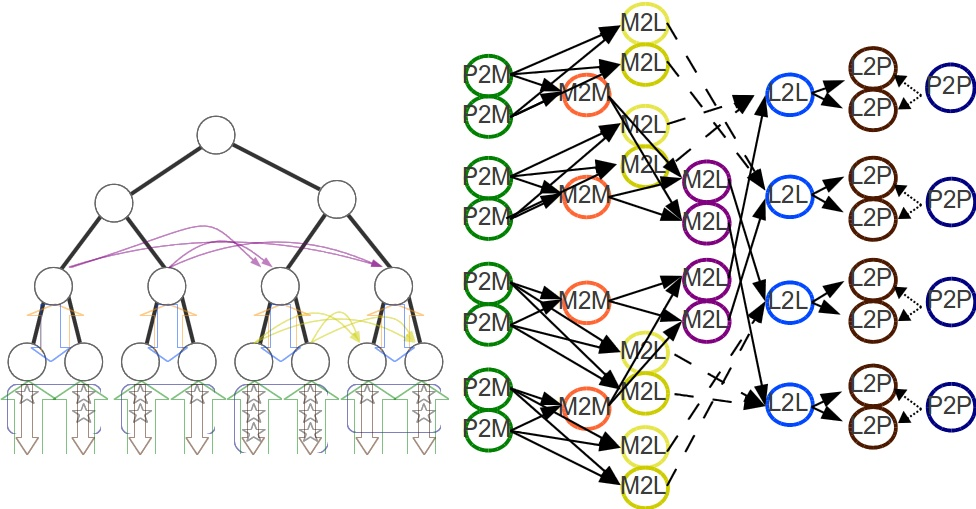
\includegraphics[width=15cm, height=15cm, keepaspectratio=true]{dag.jpg}
\caption{FMM DAG}
\end{center}
\end{figure}
%%%%%%%%%%%%%%%%%%%%%%%%%%%%%%%%%%%%%%%%%%%%%%%%%%%%%%%%%%%%%%%%%%%%
%%%%%%%%%%%%%%%%%%%%%%%%%%%%%%%%%%%%%%%%%%%%%%%%%%%%%%%%%%%%%%%%%%%%
\section{FMM Data Dependencies}
Another way to express the tasks dependencies is to express the data dependencies.
First we have to decompose the cells and particles in two parts: up and down data.
When we are transferring data in the upward pass (P2M, M2M) we are working with up/multipole part.
When we are transferring data in the downward pass (L2L, L2P) we are working with the down/local part.
Finally, the other operators (M2L, P2P) are transferring from the up part to the down part.

%%%%%%%%%%%%%%%%%%%%%%%%%%%%%%%%%%%%%%%%%%%%%%%%%%%%%%%%%%%%%%%%%%%%
%%%%%%%%%%%%%%%%%%%%%%%%%%%%%%%%%%%%%%%%%%%%%%%%%%%%%%%%%%%%%%%%%%%%
\chapter{Starpu}
\section{Introducing Starpu}
StarPU typically makes it much easier for high performance libraries or compiler environments to exploit heterogeneous multicore machines possibly equipped with GPGPUs or Cell processors: rather than handling low-level issues, programmers may concentrate on algorithmic concerns.
StarPU offers a unified offloadable task abstraction named "codelet". Rather than rewriting the entire code, programmers can encapsulate existing functions within codelets. In case a codelet may run on heterogeneous architectures, it is possible to specify one function for each architecture (e.g. one function for CUDA and one function for CPUs). StarPU takes care to schedule and execute those codelets as efficiently as possible over the entire machine. In order to relieve programmers from the burden of explicit data transfers, a high-level data management library enforces memory coherency over the machine: before a codelet starts (e.g. on an accelerator), all its data are transparently made available on the compute resource.

%%%%%%%%%%%%%%%%%%%%%%%%%%%%%%%%%%%%%%%%%%%%%%%%%%%%%%%%%%%%%%%%%%%%
%%%%%%%%%%%%%%%%%%%%%%%%%%%%%%%%%%%%%%%%%%%%%%%%%%%%%%%%%%%%%%%%%%%%
\section{Example}
In the current example, we do not use the real starpu function names.
We want to start tasks A, B and C. A works with data dt1 and dt2, B works with dt2 and dt3 and C works with dt1 and dt4.
\begin{algorithm}[H]
\restylealgo{boxed}
\linesnumbered
\SetLine
\BlankLine
StarpuInsertTask( A, READ, dt1, WRITE, dt2);
StarpuInsertTask( B, READ, dt2, WRITE, dt3);
StarpuInsertTask( C, READ, dt1, WRITE, dt4);
\BlankLine
\caption{Omp task FMM}
\end{algorithm}
\BlankLine
In the previous code, A and C can be executed simultaneously even if they both depend on dt1.
This is because they only read this data, so starpu can duplicate dt1 for each task.

%%%%%%%%%%%%%%%%%%%%%%%%%%%%%%%%%%%%%%%%%%%%%%%%%%%%%%%%%%%%%%%%%%%%
%%%%%%%%%%%%%%%%%%%%%%%%%%%%%%%%%%%%%%%%%%%%%%%%%%%%%%%%%%%%%%%%%%%%
\section{From the task to the runtime driven implementation}
As described in the previous section we express tasks dependencies by their data dependencies.
From our openmp version, with do not have many things to change.
But, even if a cell can be spited in two parts, we use one handle per cell and we do not differentiate the up part to the down part.
The same approach is used with the particles; we use one handle per leaf.
This reduces the parallelism but makes the thing much easier to code.
\BlankLine
\begin{algorithm}[H]
\restylealgo{boxed}
\linesnumbered
\SetLine
\BlankLine
\ForAll{Leaf lf in tree}{
        StarpuInsertTask( P2M, WRITE, lf.cell, READ , lf.particles )\;
}
\BlankLine
\For{idxLevel $\leftarrow$ $Height - 2$ \KwTo 1}{
        \ForAll{Cell cl at level idxLevel}{
                StarpuInsertTask( M2M , WRITE, cl, READ, cl.child)\;
        }
}
\BlankLine
\For{idxLevel $\leftarrow$ 1 \KwTo $Height - 2$}{
        \ForAll{Cell cl at level idxLevel}{
                neighbors $\leftarrow$ tree.getBoxInteractions( cl , idxLevel)\;
                StarpuInsertTask( M2L, WRITE, cl, READ, neighbors)\;
                StarpuInsertTask( L2L, READ, cl, WRITE, cl.child )\;
        }
}
\ForAll{Cell cl at level $Height - 1$}{
        neighbors $\leftarrow$ tree.getBoxInteractions( cl , $Height - 1$)\;
        StarpuInsertTask( M2L, WRITE, cl, READ, neighbors)\;
	Leaf lf as cl\;
	StarpuInsertTask( L2P, READ, cl, WRITE, lf.particles)\;
}
\BlankLine
StarpuWaitAllTask();
\BlankLine
\caption{Omp task FMM}
\end{algorithm}
\BlankLine
%%%%%%%%%%%%%%%%%%%%%%%%%%%%%%%%%%%%%%%%%%%%%%%%%%%%%%%%%%%%%%%%%%%%
%%%%%%%%%%%%%%%%%%%%%%%%%%%%%%%%%%%%%%%%%%%%%%%%%%%%%%%%%%%%%%%%%%%%
\end{document}

